\documentclass[conference]{IEEEtran}
\IEEEoverridecommandlockouts

\usepackage{cite}
\usepackage{amsmath,amssymb,amsfonts}
\usepackage{algorithmic}
\usepackage{graphicx}
\usepackage{textcomp}
\usepackage{xcolor}
\usepackage{booktabs}
\usepackage{tabularx}
\usepackage{adjustbox}
\usepackage{float}
\usepackage{ragged2e}
\usepackage[hidelinks,unicode,pdfpagelabels]{hyperref}
\usepackage[capitalise]{cleveref}

\begin{document}

\title{CodeGraph: Repository-Level Structural Retrieval for AI Coding Agents via Personalized PageRank}

\author{\IEEEauthorblockN{Alexandru-Mihai Toma}
\IEEEauthorblockA{\textit{Computer Science Department} \\
\textit{Babes-Bolyai University}\\
Cluj-Napoca, Romania \\
alexandru.toma@stud.ubbcluj.ro}
\and
\IEEEauthorblockN{Lect. Phd. Arthur Molnar}
\IEEEauthorblockA{\textit{Computer Science Department} \\
\textit{Babes-Bolyai University}\\
Cluj-Napoca, Romania \\
arthur.molnar@ubbcluj.ro}
}

\maketitle

\begin{abstract}
LLM-based coding agents can inspect files, propose patches, and run tests, but their success depends heavily on retrieving the right code context. Traditional keyword search and dense retrieval treat code mostly as text, often missing relationships expressed through imports, calls, containment, and inheritance. This paper introduces CodeGraph, a hybrid retrieval system for AI coding agents that combines lexical seeding with Personalized PageRank over a repository-level dependency graph. Evaluated on SWE-bench Lite, CodeGraph achieves 74.0\% Recall@10, a 24.3 percentage point improvement over a strong BM25-only baseline. Our empirical analysis shows that repository retrieval for AI agents improves when lexical matching is used only to place starting points, while structural propagation determines which connected code entities truly matter. The main empirical finding is that seed reachability, not ranking sophistication, sets the performance ceiling.
\end{abstract}

\begin{IEEEkeywords}
Code Retrieval, AI Agents, Graph Databases, Personalized PageRank, Static Analysis
\end{IEEEkeywords}

\section{Introduction}
\label{sec:introduction}

Autonomous coding agents require accurate context retrieval to resolve repository-level software bugs. An agent must observe the correct code files within its context window to generate valid patches. However, repositories are large and complex, and issue descriptions are written in natural language that often abstracts away from the names of classes, functions, and files.

Existing retrieval methods typically treat source code as flat text. Sparse retrievers (e.g., BM25) localize files based on term frequency but fail when the task vocabulary differs from code identifiers. Dense retrievers map natural language and code to a shared vector space, yet they compute relevance from token sequences, ignoring the structural dependencies (such as imports, calls, and inheritance) that define code execution. Consequently, text-centric methods struggle to navigate relationships that cross file and module boundaries.

Graph-based retrieval addresses these limitations by modeling the codebase as a network of entities and dependencies. In a hybrid setup, lexical search locates candidate entry points, and structural propagation traverses the graph to rank the surrounding functional neighborhood. We introduce CodeGraph, a hybrid retrieval system that integrates lexical seeding with Personalized PageRank (PPR) over a static dependency graph. In contrast to systems that rely on language models to generate queries or perform local neighborhood expansion, CodeGraph computes a global, deterministic ranking over the repository. This configuration establishes a distinct operating point: it provides repository-wide ranking under a fixed context budget without the latency or non-determinism of LLM-mediated loops.

Our central empirical finding is that seed reachability, rather than ranking sophistication, determines the retrieval ceiling. If lexical signals identify the correct general neighborhood, structural propagation reliably ranks the target files. If seeds miss the target neighborhood entirely, no ranking mechanism can recover them. 

The primary contributions of this work are:
\begin{itemize}
    \item A hybrid retrieval formulation combining multi-signal lexical seeding with global Personalized PageRank propagation to navigate repository structure.
    \item A deterministic repository-wide ranking setup that operates without placing non-deterministic language models inside the retrieval loop.
    \item An empirical evaluation on SWE-bench Lite showing a 74.0\% Recall@10, which improves upon a BM25 baseline by 24.3 percentage points.
    \item A diagnostic analysis establishing that seed reachability, rather than downstream ranking sophistication, determines the retrieval ceiling in graph-based code search.
\end{itemize}

We organize the remainder of this paper as follows. \Cref{sec:related_work} positions CodeGraph against sparse, dense, and graph-based retrieval. \Cref{sec:method} details the core retrieval methodology. \Cref{sec:system} provides an overview of the system architecture. \Cref{sec:experimental_setup} outlines the evaluation framework, and \Cref{sec:results} reports the quantitative findings. \Cref{sec:discussion} analyzes the structural limits and implications for coding agents, and \Cref{sec:conclusion} concludes.

\section{Related Work}
\label{sec:related_work}

Code retrieval methods for large language models generally fall into three categories: sparse lexical search, dense vector retrieval, and graph-based traversal.

\textbf{Sparse Retrieval:} Sparse methods like BM25 \cite{bm25} rank files based on term frequency overlap. Although highly scalable and deterministic, sparse methods are sensitive to exact lexical matches. They struggle when natural-language descriptions use abstract terminology that does not match specific code identifiers.

\textbf{Dense Retrieval:} Dense retrieval models like CodeBERT \cite{codebert} and UniXcoder \cite{unixcoder} embed queries and code snippets into a continuous vector space to capture semantic similarity. While this helps bridge vocabulary differences, dense models ignore the explicit structural dependencies that govern program execution. Dense models do not encode inheritance or call relationships directly, and their vector similarity scores provide no interpretable trace for debugging context selection. CodeGraph is designed as a hybrid system: lexical and dense methods can identify starting points, while graph propagation performs structural ranking.

\textbf{Graph-Based Retrieval:} Graph-based systems represent source repositories as networks of program entities and dependencies. Table~\ref{tab:retrieval-comparison} compares CodeGraph with representative systems on graph granularity, retrieval method, ranking scope, and computational cost.

\begin{table}[htbp]
    \centering
    \caption{Comparison of repository retrieval approaches.}
    \label{tab:retrieval-comparison}
    \begin{adjustbox}{max width=\linewidth}
    \begin{tabular}{lllll}
        \toprule
        \textbf{System} & \textbf{Graph Level} & \textbf{Retrieval Method} & \textbf{Global Ranking} & \textbf{Deterministic \& Low-Cost} \\
        \midrule
        BM25 \cite{bm25} & None & Term matching & Yes & Yes \\
        CodeBERT \cite{codebert} & None & Vector similarity & Yes & Yes \\
        \midrule
        RepoGraph \cite{ouyang2025repograph} & Line & $k$-hop ego-graph & None & Yes \\
        LocAgent \cite{chen2025locagent} & Entity & BFS + BM25 rescoring & Local & Yes \\
        CodexGraph \cite{liu2024codexgraph} & Symbol & LLM graph queries & None & No \\
        LARGER \cite{hu2026larger} & Entity & Local expansion & Local & Yes \\
        \midrule
        \textbf{CodeGraph} (Ours) & Entity & Lexical seeds + PPR & \textbf{Global} & \textbf{Yes} \\
        \bottomrule
    \end{tabular}
    \end{adjustbox}
\end{table}

Existing graph systems face distinct design trade-offs:
\begin{itemize}
    \item \textbf{RepoGraph} \cite{ouyang2025repograph} models code at the line level and extracts unranked $k$-hop ego-graphs. Because it lacks a ranking function, expanding the traversal radius returns large, unfiltered code blocks that consume the agent's context budget.
    \item \textbf{LocAgent} \cite{chen2025locagent} and \textbf{LARGER} \cite{hu2026larger} combine lexical search with local graph traversal. However, they limit expansion to local neighborhoods and do not compute a global repository-wide ranking.
    \item \textbf{CodexGraph} \cite{liu2024codexgraph} uses a language model to generate graph-database queries. Placing an LLM inside the retrieval loop increases query latency, monetary cost, and non-deterministic behavior.
\end{itemize}

CodeGraph differs from these approaches by combining multi-signal lexical matching for seed selection with Personalized PageRank (PPR) for global repository ranking. This design yields a deterministic, low-cost retrieval method that evaluates execution-level structures to deliver a ranked context package under a fixed budget.

\section{Methodology}
\label{sec:method}

CodeGraph separates repository retrieval into two explicit responsibilities: lexical signals identify plausible entry points into the codebase, while structural propagation computes the final ranking over reachable code entities. This division of labor is central to the method. Natural-language issue text is used only to place initial probability mass, whereas the ranking itself is determined by repository structure, making retrieval reproducible, interpretable, and aligned with execution semantics. CodeGraph separates computation into two stages: the Indexing Phase constructs the repository graph once, and the Retrieval Phase performs seed selection, graph propagation, and ranking for each query.

\subsection{Seed Selection}

Personalized PageRank requires a set of starting nodes. Seed selection translates the natural-language task description into a personalization vector: a probability distribution determining where the random walk restarts.

CodeGraph constructs this vector from three complementary signals:
\begin{enumerate}
    \item \textbf{Entity match:} Entity match identifies explicit code-like mentions in the task description, including CamelCase and snake\_case identifiers, and maps them directly to nodes in the graph vocabulary. This signal captures cases where the issue text already names a relevant program entity, but it is moderated with inverse-document-frequency (IDF) scaling so that highly ambiguous identifiers, such as common verbs or generic class names, do not dominate the personalization vector.
    \item \textbf{BM25 keyword search:} BM25 keyword search broadens coverage when the issue description does not contain an exact identifier match. Each entity is indexed by its short name, qualified name, file path, and docstring content, allowing lexical relevance to be estimated over multiple views of the same code object. To reduce vocabulary mismatch, compound tokenization splits identifiers at CamelCase boundaries and underscores, so abstract phrases such as ``SQL compilation'' can still recover composite names such as \texttt{SQLCompiler}.
    \item \textbf{Issue path hint:} Issue path hints exploit references to directory names or file names that appear directly in the task description. When such fragments are present, they are mapped to entities under the corresponding repository path, allowing the seed set to be biased toward the relevant module even when the issue text does not explicitly name the final target entity.
\end{enumerate}

These signals are merged to form a robust starting distribution that does not rely exclusively on perfect entity resolution. For example, an issue may mention ``SQL compilation'' without naming the exact implementation file. Compound tokenization allows this phrase to match identifiers such as \texttt{SQLCompiler}, path hints can bias the search toward the relevant module, and the resulting seed set gives Personalized PageRank a structurally meaningful region from which to begin propagation.

\subsection{IDF-Based Edge Reweighting}

Uniform graph traversal assumes every structural connection contributes equally to relevance. In practice, however, some connections point to highly specific domain logic, while others point to generic utility nodes (e.g., global loggers or base classes) reused across large parts of the repository.

To attenuate the influence of generic hubs, CodeGraph assigns each edge a weight inversely proportional to the in-degree of its target node: 
\begin{equation}
    w(e) = \frac{1}{\log_2(\operatorname{in\_degree}(v) + 2)}
    \label{eq:idf-weight}
\end{equation}
This logarithmic penalty steers probability mass away from ubiquitous hubs, ensuring that relevance is propagated primarily along domain-specific pathways. \Cref{fig:idf-reweighting} illustrates this intuition.

\begin{figure}[htbp]
    \centering
    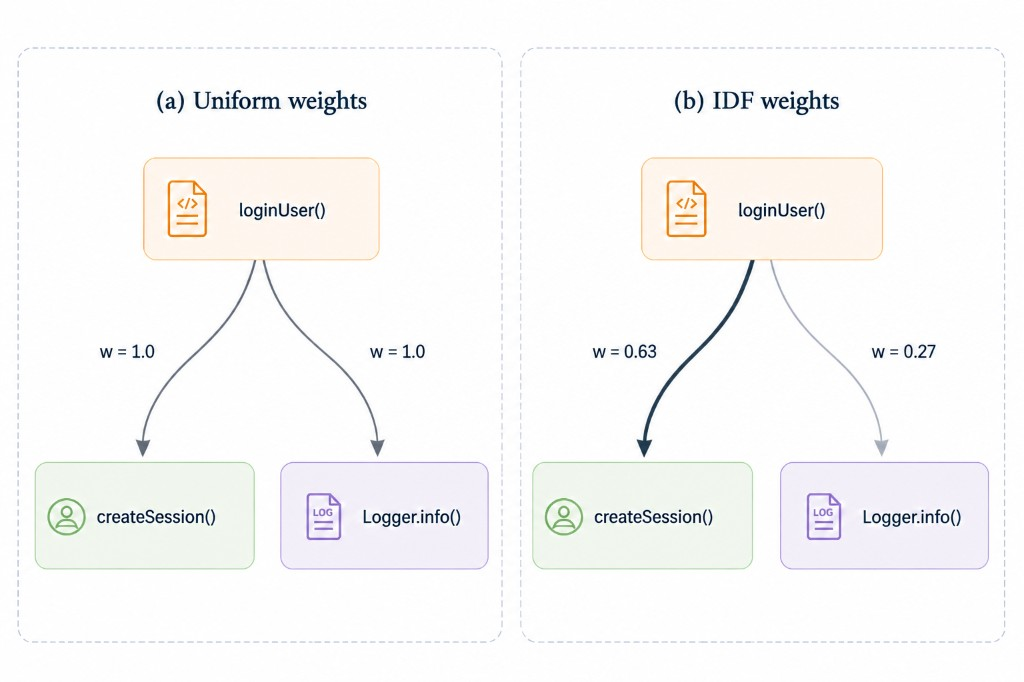
\includegraphics[width=\linewidth]{assets/idf_reweighting.png}
    \caption{IDF edge reweighting. Panel (a) uses uniform weights, diluting relevance. Panel (b) attenuates the weight toward the high in-degree hub, keeping relevance mass on the domain-specific callee.}
    \label{fig:idf-reweighting}
\end{figure}

\subsection{Personalized PageRank Propagation}

With the seed personalization vector $\vec{s}$ and the edge weights $w(e)$ defined, relevance is propagated through the graph using Personalized PageRank (PPR) \cite{jeh2003ppr}. The stationary relevance vector $\vec{r}$ is computed as the solution to:
\begin{equation}
    \vec{r} = (1 - d) \vec{s} + d P^T \vec{r}
    \label{eq:ppr}
\end{equation}
where $d \in (0,1)$ is the damping factor (set to $0.70$), and $P$ is the transition probability matrix. The transition probability from node $u$ to node $v$ is normalized over outgoing edges using the IDF-reweighted values:
\begin{equation}
    P_{uv} = \frac{w(u, v)}{\sum_{(u, k) \in E} w(u, k)}
    \label{eq:transition}
\end{equation}
We compute Personalized PageRank over an undirected projection of the property graph, allowing relevance mass to diffuse both upstream (from callees to callers) and downstream (from callers to callees). This bidirectional propagation is intentional: an issue may describe a callee, a caller, or a related imported component, so retrieval must move in both directions across the dependency graph to recover the correct structural neighborhood. The resulting vector $\vec{r}$ provides a topologically anchored relevance score for every code entity in the repository.

\subsection{Methodological Commitments}

CodeGraph is defined not only by its use of Personalized PageRank, but by four methodological commitments that shape how relevance is represented and propagated through the repository graph.

\textbf{Coarse-Grained Entity Granularity:} The graph schema restricts nodes strictly to files, classes, functions, and methods. CodeGraph explicitly avoids line-level resolution or full Abstract Syntax Tree (AST) ingestion. While ASTs capture complete syntactic correctness, their overwhelming density dilutes retrieval probability mass. The chosen four-entity model provides the exact abstraction layer through which developers typically organize, modularize, and reference code, maintaining a graph size that is efficient for matrix operations.

\textbf{Precision Over Noisy Connectivity:} During graph construction, we resolve calls conservatively. If a function call site is ambiguous and cannot be resolved to a definitive definition within the codebase, CodeGraph omits the edge entirely. This choice favors precision over recall in the graph topology itself: it is safer to miss an implicit connection than to inject false structural pathways that would misdirect the PageRank random walk. 

\textbf{Explicit Dependencies Over Proximity Heuristics:} We restrict edges strictly to syntactic dependencies (\texttt{CALLS}, \texttt{IMPORTS}, \texttt{CONTAINS}, \texttt{INHERITS\_FROM}). We do not use directory-proximity heuristics (e.g., connecting all files in the same folder), as adding proximity edges creates dense subgraphs that indiscriminately diffuse relevance. CodeGraph's retrieval fidelity is built on the premise that execution paths matter more than file system locality.

\textbf{Uniform Restart as a Robustness Mechanism:} A critical algorithmic decision is the use of a uniform restart distribution over the selected seeds, rather than weighting restarts by lexical confidence scores. In software repositories, a highly confident lexical match is often an ambiguous, common identifier (e.g., a generic \texttt{Manager} class). Weighting by confidence amplifies these false positives. Uniform restart is a robustness decision under noisy seed conditions: by giving every extracted seed an equal share of the initial mass, CodeGraph allows the graph topology to arbitrate. Correct seeds that share structural paths compound their mass cooperatively, while isolated incorrect seeds dissipate their relevance into uncoordinated neighborhoods. Taken together, these design choices define CodeGraph as a deterministic repository-level retrieval system in which lexical signals identify entry points and graph propagation determines the final ranking.

\section{System Overview}
\label{sec:system}

CodeGraph formulates repository retrieval as a staged transformation from raw source code to ranked context. The pipeline comprises parsing, graph construction, seed selection, PPR-based ranking, and context delivery. \Cref{fig:pipeline-architecture} illustrates this workflow. By separating graph construction (offline) from retrieval (online), the system guarantees deterministic, low-latency responses suitable for agent integration.

\begin{figure}[htbp]
    \centering
    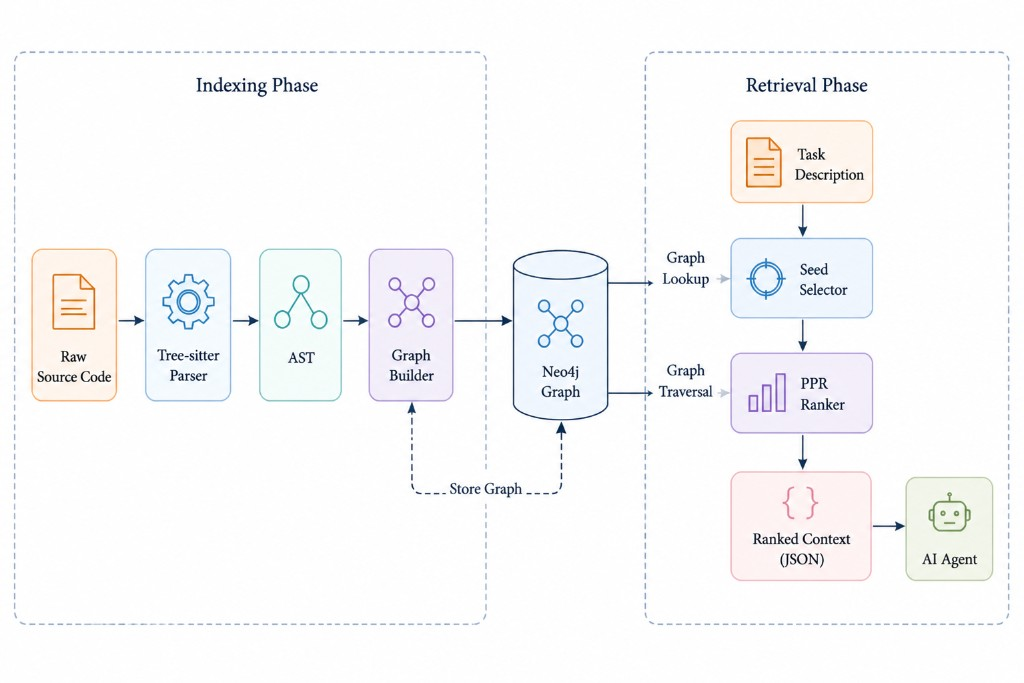
\includegraphics[width=\linewidth]{assets/pipeline_architecture.png}
    \caption{CodeGraph indexing and retrieval pipeline. The indexing phase builds the repository graph offline; the retrieval phase ranks context per query for the AI agent.}
    \label{fig:pipeline-architecture}
\end{figure}

\subsection{Graph Representation}

Graph-based retrieval requires an explicit structural representation of the repository. CodeGraph uses Tree-sitter \cite{treesitter} to extract a four-entity model: files, classes, functions, and methods. This granularity captures the units through which Python code is typically referenced while preserving a graph size that remains efficient for matrix operations.

CodeGraph stores these entities as a property graph in Neo4j \cite{neo4j2024docs}, using four edge types (\texttt{CONTAINS}, \texttt{CALLS}, \texttt{IMPORTS}, and \texttt{INHERITS\_FROM}) to capture the main structural patterns of a Python codebase (\Cref{fig:graph-schema}). Call resolution favors precision over recall by omitting ambiguous call sites, ensuring that graph pathways reflect genuine structural dependencies rather than false positive links.

\begin{figure}[htbp]
    \centering
    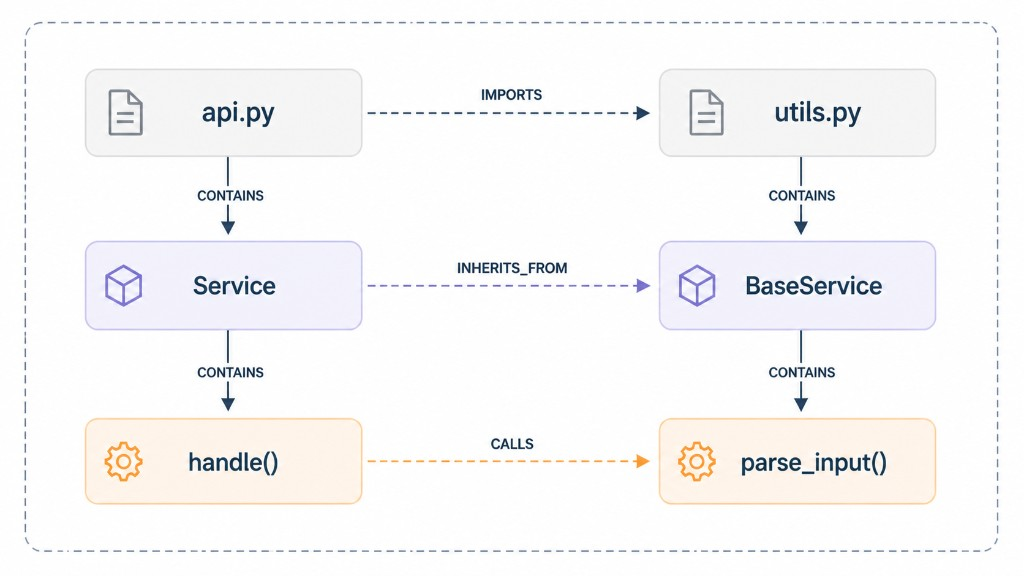
\includegraphics[width=\linewidth]{assets/graph_schema.png}
    \caption{CodeGraph property-graph schema. Nodes represent fundamental code units; edges capture containment, linkage, extension, and invocation.}
    \label{fig:graph-schema}
\end{figure}

\subsection{Context Delivery}

Once the PPR algorithm ranks the graph, the result must be packaged into a fixed context budget. CodeGraph post-processes the ranked nodes by deduplicating entities from the same file, dropping parent \texttt{File} nodes if specific sub-entities (like a method) are already highly ranked, and extracting the corresponding source text. 

The entire retrieval pipeline is wrapped into a Model Context Protocol (MCP) server. This exposes a single \texttt{get\_relevant\_context} tool, allowing AI agents to programmatically fetch ranked, budget-constrained source snippets deterministically, avoiding the latency and instability of LLM-generated graph queries inside the retrieval loop.

\section{Experimental Setup}
\label{sec:experimental_setup}

We evaluate CodeGraph on SWE-bench Lite \cite{yang2024swebench}, a benchmark consisting of 300 real GitHub issues from 12 open-source Python repositories. The objective is repository-level retrieval: given only a natural-language issue description, the system must rank files by relevance, placing the files modified in the human patch at the top of the ranked list.

\subsection{Metrics and Protocol}

Although Personalized PageRank propagates relevance over fine-grained structural entities (classes, functions, and methods), we evaluate retrieval performance at the file level. File-level retrieval serves as the correct proxy for agent context acquisition, as coding agents typically load entire files into their context window to preserve syntactical context.

To map entity-level scores to file-level ranks, we group the ranked entities by their parent file and assign each file the score of its highest-ranked constituent entity. We measure performance using three metrics:
\begin{itemize}
    \item \textbf{Recall@$k$ (R@$k$):} The fraction of issues where the target file is retrieved within the top-$k$ results. R@10 is our primary metric, reflecting the typical context budget of AI coding agents.
    \item \textbf{Mean Reciprocal Rank (MRR):} The average of $1 / \operatorname{rank}$ for the target file, indicating the precision of the ranked results.
    \item \textbf{Zero-recall count:} The number of issues where the target file does not appear in the top-10 results, indicating a reachability failure.
\end{itemize}

\subsection{Baselines}

We evaluate CodeGraph against four baseline configurations to isolate the contributions of lexical matching, graph topology, and ranking propagation:
\begin{enumerate}
    \item \textbf{BM25-only (Basic):} A sparse lexical retriever executing over the entity signatures and docstrings. This baseline omits the dependency graph entirely, serving as a measure of standard text search.
    \item \textbf{One-hop ego graph:} A structural baseline that retrieves all nodes within a single hop of the BM25 seed nodes without ranking. This tests whether graph structure alone is sufficient without PageRank propagation.
    \item \textbf{CodeGraph (Initial):} An early system configuration that applied confidence-weighted PPR restart, representing the performance of graph-based ranking prior to our seed engineering interventions.
    \item \textbf{BM25-only (Seed-Engineered):} A lexical baseline that uses our optimized seed corpus (including compound tokenization and path hints) but omits PPR propagation, isolating the value of structural routing.
\end{enumerate}

\section{Results and Analysis}
\label{sec:results}

\subsection{Main Benchmark Comparison}

The final CodeGraph configuration achieves \textbf{74.0\% Recall@10}, an absolute improvement of 24.3 percentage points over the strong BM25-only baseline. \Cref{tab:main-results} presents the final comparative evaluation. Because the retrieval pipeline relies on deterministic algorithms (static parsing, BM25 matching, and exact PageRank calculation), these results are stable and not subject to the statistical variance that affects LLM-mediated retrieval loops.

\begin{table}[htbp]
    \centering
    \caption{Main quantitative comparison on SWE-bench Lite (300 instances).}
    \label{tab:main-results}
    \begin{adjustbox}{max width=\linewidth}
    \begin{tabularx}{\linewidth}{@{} >{\RaggedRight\arraybackslash}X >{\RaggedRight\arraybackslash}p{1.2cm} >{\RaggedRight\arraybackslash}p{1.2cm} >{\RaggedRight\arraybackslash}p{1.2cm} >{\RaggedRight\arraybackslash}p{1.6cm} @{}}
        \toprule
        \textbf{Method} & \textbf{R@5} & \textbf{R@10} & \textbf{MRR} & \textbf{Zero-recall} \\
        \midrule
        BM25-only Baseline & 37.7\% & 49.7\% & 0.248 & 151 \\
        CodeGraph (Initial) & 37.0\% & 42.0\% & 0.228 & 174 \\
        \textbf{CodeGraph (Final)} & \textbf{60.7\%} & \textbf{74.0\%} & \textbf{0.442} & \textbf{78} \\
        \bottomrule
    \end{tabularx}
    \end{adjustbox}
\end{table}

\subsection{Engineering Trajectory and Ablation}

The initial configuration of CodeGraph (42.0\% R@10) underperformed the lexical baseline. The final result (74.0\% R@10) was reached through systematic refinement of the seed stage (\Cref{fig:trajectory}).

\begin{figure}[htbp]
    \centering
    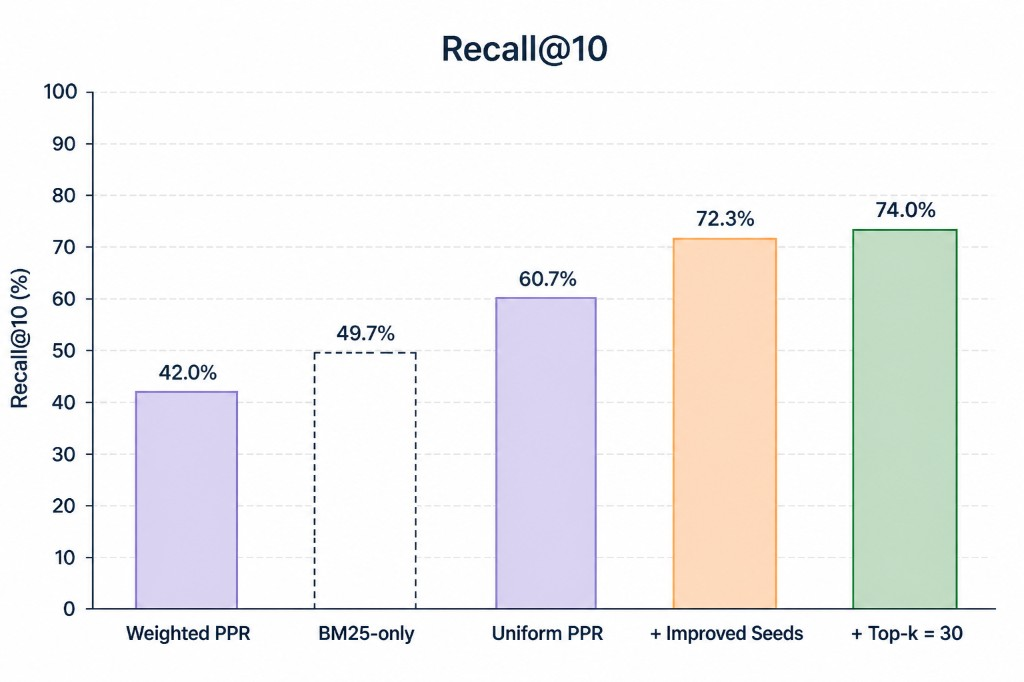
\includegraphics[width=\linewidth]{assets/recall_trajectory.png}
    \caption{Recall@10 engineering trajectory. Successive algorithmic and lexical refinements recovered the initial performance deficit and surpassed the lexical baseline.}
    \label{fig:trajectory}
\end{figure}

The improvement breaks down into three sequential interventions:
\begin{enumerate}
    \item \textbf{Algorithm Refinement (+18.7pp):} Switching from confidence-weighted to uniform PPR restart closed the gap with BM25. When seeds are noisy, assigning them proportional weights amplifies false positives. Uniform restart allows the graph topology itself to arbitrate relevance through path convergence.
    \item \textbf{Seed Engineering (+11.6pp):} Implementing compound tokenization, an expanded BM25 corpus, and IDF entity weighting ensured that task descriptions resolved to structurally meaningful starting nodes.
    \item \textbf{Budget Adjustment (+1.7pp):} Increasing the output threshold from 20 to 30 files recovered instances where the target was correctly identified but ranked just outside the initial cutoff.
\end{enumerate}

To test the schema's reliance on explicit dependencies, we conducted an ablation that augmented the graph with \texttt{CO\_LOCATED} proximity edges between sibling files. This caused a 1.0pp regression: artificial density dilutes relevance across unrelated files, proving that CodeGraph's precision derives strictly from high-fidelity dependency links rather than structural heuristics.

\subsection{The Reachability Bottleneck}

A defining characteristic of CodeGraph is its bimodal rank distribution: the target file almost always lands in the top-5 or does not appear in the top-10 at all. As \Cref{fig:bimodal} shows for the initial configuration, only 5\% of instances fell into the intermediate band (ranks 6--10).

\begin{figure}[htbp]
    \centering
    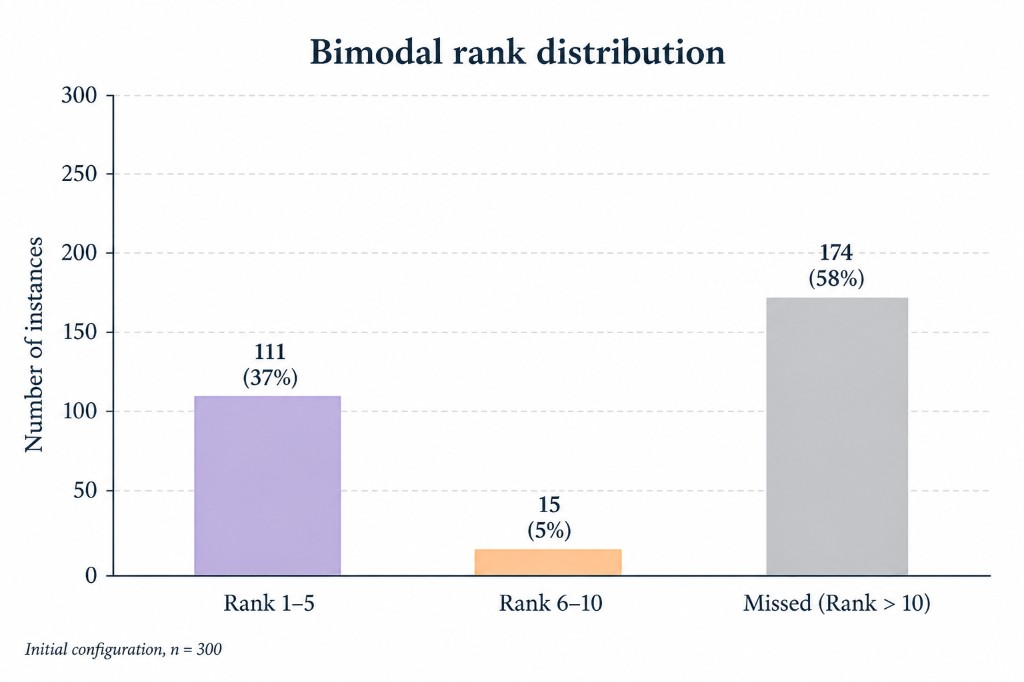
\includegraphics[width=\linewidth]{assets/bimodal_rank_distribution.png}
    \caption{Bimodal rank distribution for the initial configuration. The near-absence of intermediate ranks indicates that Reachability is the primary bottleneck.}
    \label{fig:bimodal}
\end{figure}

This pattern yields our central empirical finding: the retrieval ceiling is bounded by Reachability, not Ranking. If the system retrieves the target file at all, the PPR algorithm ranks it highly. The zero-recall failures occur exclusively when no seed lies on a structurally connected path to the target. When seeds miss the relevant neighbourhood entirely, the graph has no signal to propagate. This diagnostic directly motivated our emphasis on seed quality engineering rather than advanced ranking heuristics.

\subsection{Qualitative Retrieval Cases}

To illustrate how the hybrid mechanism operates in practice, we examine two representative retrieval episodes: one success and one failure.

\textbf{Success Case (Structural Amplification):} In \textit{matplotlib/matplotlib-23562}, the bug report requests support for a new 3D surface attribute. The issue text briefly mentions \texttt{Poly3DCollection}. The lexical index correctly identifies \texttt{Poly3DCollection} as a seed, but it also falsely matches generic terms like \texttt{color} and \texttt{facecolors} across dozens of unrelated files. During structural propagation, the generic seeds dissipate their probability mass across disparate, disconnected utility modules. Conversely, the specific seed \texttt{Poly3DCollection} propagates its mass locally through direct \texttt{CALLS} and \texttt{INHERITS\_FROM} edges. The target file, \texttt{lib/mpl\_toolkits/mplot3d/art3d.py}, absorbs this concentrated mass and is ranked at position 1. This demonstrates graph topology successfully filtering out lexical noise.

\textbf{Failure Case (Semantic Gap):} In \textit{django/django-11001}, the user describes a bug where ``raw SQL queries containing multi-line strings cause a syntax error.'' The description is entirely conceptual and uses no actual Django source-code identifiers. Because the words ``raw'', ``SQL'', and ``syntax'' do not uniquely match the specific compiler classes responsible for the bug (e.g., \texttt{SQLCompiler} in \texttt{django/db/models/sql/compiler.py}), the lexical stage fails to extract any meaningful seeds. Without a localized entry point, PPR cannot traverse the relevant dependency subgraph, resulting in a zero-recall failure. This case perfectly illustrates the structural ceiling: no amount of sophisticated graph routing can compensate for a total failure to enter the correct structural neighbourhood.

\section{Discussion and Limitations}
\label{sec:discussion}

The main value of CodeGraph is not only that it improves retrieval accuracy, but that its failure modes are structurally interpretable. Because ranking is deterministic and graph-constrained, missed targets can be traced to missing reachability rather than opaque model behavior. This makes the remaining limitations scientifically informative, and also suggests where hybrid retrieval systems should focus future effort.

\subsection{Practical Implications for AI Coding Agents}

For AI coding agents to operate autonomously, they require retrieval tools that are not only accurate but stable. When an agent requests context, it needs a fast, predictable response. Systems that place large language models directly inside the retrieval loop (e.g., to generate graph queries or re-rank snippets) introduce high latency and non-deterministic variance. An agent debugging a failure may receive a different context window upon retrying the exact same task.

CodeGraph provides a deterministic foundation for agent memory. By separating the graph construction (performed asynchronously) from the ranking phase (performed via deterministic matrix multiplication), the system guarantees that the same seed set will always produce the exact same topological ranking. This allows agent designers to cache results, write reproducible evaluation harnesses, and treat the repository graph as a stable environment rather than a stochastic oracle.

\subsection{Structural Limitations and Future Hybridization}

An analysis of the zero-recall instances defines the exact boundaries of static graph-based retrieval. We identify two primary failure modes (\Cref{fig:taxonomy}):

\begin{figure}[htbp]
    \centering
    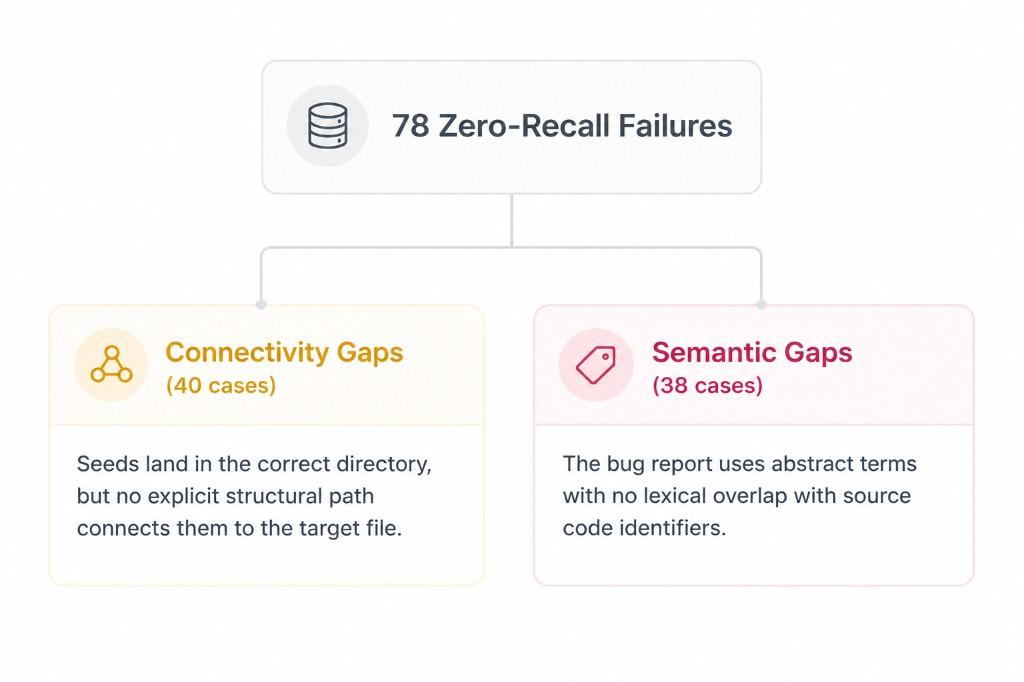
\includegraphics[width=\linewidth]{assets/failure_taxonomy.png}
    \caption{Failure taxonomy of the zero-recall instances. Connectivity Gaps account for 40 cases (missing graph edges), and Semantic Gaps account for 38 cases (lexical mismatch).}
    \label{fig:taxonomy}
\end{figure}

\textbf{Connectivity Gaps (40 instances):} These occur when seeds land in the correct general region, but no explicit syntactic dependency (e.g., \texttt{CALLS} or \texttt{IMPORTS}) connects the seed to the specific target file. Files that collaborate through implicit data flows, configuration files, or dynamic plugin registries remain invisible to standard structural propagation. This establishes the ceiling of purely static graph retrieval.

\textbf{Semantic Gaps (38 instances):} These failures arise when the issue description uses highly abstract natural-language terms with zero lexical overlap with any source-code identifier. Without a lexical anchor, the system cannot place any seed in the relevant neighbourhood, causing a total reachability failure.

These limitations naturally motivate the next stage of hybridization. To bridge semantic gaps without sacrificing determinism, future systems should investigate employing lightweight dense embeddings strictly for the initial seed selection stage, allowing abstract tasks to anchor correctly before delegating the final ranking back to the graph structure. To bridge connectivity gaps, integrating dynamic execution traces or semantic data-flow edges could expose implicit dependencies that static syntax misses, yielding an even more complete topological view of the repository.

\section{Conclusion}
\label{sec:conclusion}

This paper introduced CodeGraph, a hybrid retrieval system for AI coding agents that bridges the gap between natural-language task descriptions and repository-level source code. By extracting lexical seeds and propagating relevance over a static dependency graph using Personalized PageRank, CodeGraph achieves 74.0\% Recall@10 on the SWE-bench Lite benchmark.

The central finding of this work is that structural retrieval performance is primarily bottlenecked by Reachability, not Ranking. When lexical signals identify even a noisy starting point, the graph topology reliably arbitrates relevance and pushes correct files to the top. The Seed-First engineering strategy (incorporating uniform PPR restart, compound tokenization, and IDF edge weighting) outperformed the lexical baseline by 24.3 percentage points.

Future work should target the remaining Connectivity and Semantic Gaps. Dense embedding models could replace sparse matching to better map abstract language to starting nodes, while lightweight dynamic tracing could expose the implicit dependencies that static analysis misses. Ultimately, CodeGraph demonstrates that repository retrieval improves when text matching is constrained to finding starting points, while deterministic graph propagation identifies the code that truly matters.


\nocite{*}
\bibliographystyle{IEEEtran}
\bibliography{references}

\end{document}
